\subsection{Erkentnisse aus der Inbetriebnahme}\label{sec:energieuebertragung}

Der erste Prototyp der Pulsschaltung für die Induktion wurde mithilfe eines NE555 realisiert. Dabei wurden als Widerstände Potentiometer eingebaut, mit welchen die Resonanzfrequenz des LC-Gliedes gesucht werden sollte.

Der allererste Versuch ergab eine Übertragung von 5mA bei einer Taktfrequenz von 10kHz. Es stellte sich relativ schnell heraus, dass die Taktfrequenz viel zu tief war. Das konnte festgestellt werden indem man die Taktfrequenz der Pulsschaltung veränderte. So ergab sich das bei höherer Taktfrequenz die Übertragung besser wurde.

Da die Taktfrequenz der NE555-Prototypenschaltung aufgrund der Potentiometer Wahl auf 10kHz begrenzt war. Wurde nun in weiteren schritten mit dem Frequenzgenerator der 2n3055 Leistungstransistor angesteuert. Des Weiteren wurde das C aus dem LC-Glied ausgebaut, um so das spezifische maximum der Spule zu finden.

So wurde nun mit konstanter Eingangsspannung und variabler Taktfrequenz die Spule ausgetestet. Es zeichnete sich folgendes Bild ab. Mit höher werdender Frequenz wurde die Übertragung besser. Um diese noch weiter zu verbessern empfiehlt sich bei der Taktfrequenz einen Dutycycle von möglichst 50% zu erzielen.

Es erwiess sich, dass bei der Taktfrequenz von 93kHz die beste Übertragung zustande kam. Bei höheren Frequenzen war diese wieder Rückläufig. Nun da die optimale Frequenz gefunden und die Induktivität der Spule bekannt war (14.9 H) konnte der ideale Kopplungskondensator berechnet werden. Dies ergab, unter Berücksichtigung der E-Reihen, einen 220nF Kondensator als ideal. Damit die Spule nicht zu heiss werden konnte und dadurch ihren Isolierlack begann zu schmelzen, wurde der Strombegrenzungswiderstand des 2n2222 mit 2 Ohm definiert. Die Berechnung hierzu ist im oberen Text zu finden.

Somit sind alle benötigten Bauteile bekannt.

\begin{figure}[H]
	\begin{center}
		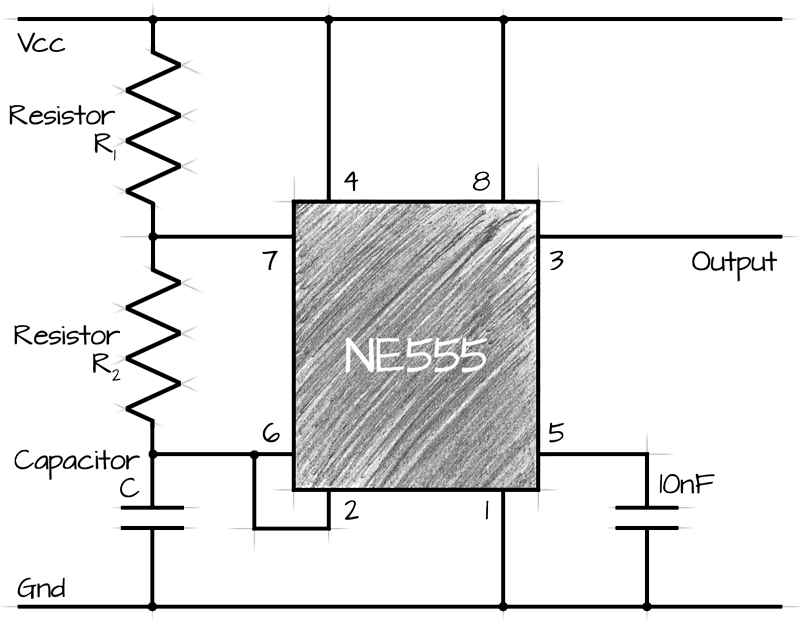
\includegraphics[width=80mm]{data/Ne555circuit.png}
		\caption[Ne555]{Die verwendete Timerschaltung als Pulsquelle} %picture caption
		\label{fig:Prototyp Down}
	\end{center}
\end{figure}

\begin{center}
C: 1nF
R1: 200 Ohm
R2:9 kOhm
\end{center}

Mit diesen Werten konnte nach dem Gleichrichter, bei einer Übertragungsdistanz von einer Standard-Platinen dicke, eine Leerlaufspannung von ca. 17V und ein Kurzschlussstrom ca. 300mA gemessen werden. Es gilt jedoch zu beachten, dass diese Werte ohne Last gemessen wurden. 

Da nun die Induktionsstufe funktioniert wird diese nun um die Ladeschaltung erweitert. Hier ergab sich folgendes Problem:

Die Eingangsspannung des Lade-Ic’s darf nicht mehr als 6.5 Volt betragen. Da die Receiverspule sich im inneren des Dojo’s befindet und dadurch nur eine sehr geringe Baugrösse besitzen darf, kann diese zwangsläufig keine grossen Leistungen erbringen. Dies bedeutet, dass akzeptabel Ladeströme nur mit genügend hohen Spannungen erzeugt werden können.

Um dies zu erzielen wurde versucht, einen Spannungsregler einzubauen, um den übertragenen Strom bei zuhalten, jedoch die Spannung zu begrenzen. Das Ergebnis davon war jedoch ziemlich bescheiden. Der so entstehende Energieverlust ist ziemlich gross und ausserdem kam es vereinzelt vor, dass der Lade ic trotzdem kaputt ging, da der Spannungsregler nicht sauber regelte. 

Die Ideale Lösung wäre natürlich einen geeigneteren Lade-Ic zu nehmen. Da jedoch die Validierung desjenigen bereits durchgeführt wurde und nicht genügend Zeit vorhanden war diesen erneut zu bestellen wurde sich entschieden die Transceiver Schaltung ein wenig anzupassen.

Dabei gibt es folgende Möglichkeiten. Man kann die Eingangsspannung absenken. Dies beeinflusst jedoch auch den Übertragenen Strom exponentiell, da einerseits eingangsseitig mit weniger Spannung auch weniger Strom durch die Spule fliess und andererseits auch der Leistungsstransistor nicht sauber durchgesteuert wird da dieser ebenfalls an der gleichen Versorgungsspannung hängt und somit sein Pulssignal beeinflusst. Die zweite Möglichkeit ist die Taktfrequenz verringern. Dadurch wird die Induzierte Spannung ebenfalls abgesengt was ebenfalls den Strom exponentiell beeinflusst. Die dritte Möglichkeit wäre die Übertragungsdistanz zu verringern. Da aber sichergestellt werden wollte, dass der Dojo-Boden dennoch eine gewisse Stabilität aufweisen sollte wurde diese Distanz der Platinendicke beigehalten.

Somit wurde die Schaltung lange ausgetestet um die beste Kombination zu erzielen. Das beste Resultat ergab die Kombination zwischen einer Taktfrequenz von ca 80kHz und einer Eingangs Spannung von 8.3V. Dies lässt sich damit erklären das leichtes Absenken der beiden Möglichkeiten den Strom nicht so stark beeinflusst. Des Weiteren wurde der Strombegrenzungswiderstand auf 1.5 Ohm verringert da sich die Eingangs Spannung verringert hat und ausserdem der Stromfluss durch die Spule damit erhöht wurde. 

Diese Anpassungen fielen ebenfalls zu Gunsten des Energiemanagements, jedoch ist dies eine stabile Variante für die ersten Prototypen. Durch die Anpassungen wird die überschüssige Energie in Form von Wärme an dem Transceiver Spule abgegeben. Die Test ergaben, dass so die Batterie bei einer Spannung von 4.7V mit 70mA geladen wird. Es ist ebenfalls möglich kurzzeitig mit einem höheren Strom zu laden, wenn die Eingangs Spannung nur geringfügig erhöht wird. (bis zu 120mA). Jedoch ist die Hitzeentwicklung hierbei so gross, dass nach einer gewissen Zeit die Übertragung zusammenbricht. Deshalb ist zu empfehlen die angegebenen Werte nicht zu überschreiten um eine dauernde Funktionalität zu gewährleisten.

Die Werte der oben beschriebenen angepassten Pulsschaltung sind folgende:
C: 1nF\\
R1: 200 Ohm\\
R2:9 kOhm\\

\subsection{optimierungsmöglichkeiten für die nächsten Varianten}\label{sec:energieuebertragung}
Für nachfolgende Weiterentwicklungen der Ladestufe empfiehlt es sich, einen Lade-IC zu verwenden, welcher eine grössere Eingangsspannung verarbeiten kann. Bei einer Recherche wurde dieses Modell herausgesucht: AAAAAAAAAAAAAAA.

Desweiteren würde es sich Lohnen die Spulen zu optimieren. Die eingebauten Flachspulen sind zwar platzsparen, kommen jedoch aufgrund ihrer Bauform ziemlich schnell an ihr Leistungsmaximum. Hier würden sich solche Spulen sich empfehlen, wie sie z.B. auch in modernen elektrischen Zahnbürsten verwendet werden. Hierbei handelt es sich um zwei unterschiedlich grosse Ringspulen, von welchem die kleinere Tranceiver-Spule in der Ladeschaltung in die grössere Receiverspule  im Dojo gesteckt wird. Diese Ringspulen wären zwar ein wenig grösser, doch durch die grössere Bauform könnte die Ladeschaltung mit grösseren Strömen betrieben und damit auch der Dojo noch schneller geladen werden.